
\section{Ключевые алгоритмы и формулы}

\subsection{Алгоритм разбиения текста на фрагменты (Text Chunking)}

Первым этапом конвейера индексации является разбиение извлечённого из документа текста на фрагменты — чанки. Прямая передача документа целиком в модель эмбеддингов невозможна по двум причинам. Во-первых, языковые и эмбеддинговые модели имеют ограничения на максимальную длину входной последовательности токенов, и длинный документ может просто не поместиться в контекст. Во-вторых, даже если технически передать документ целиком, это нецелесообразно с точки зрения точности поиска: векторное представление большого текста неизбежно усредняет семантику всех содержащихся в нём тем, что резко снижает точность при сопоставлении с конкретным, узко сформулированным запросом пользователя.

В разрабатываемой системе применяется стратегия рекурсивного посимвольного разбиения (Recursive Character Text Splitting). Алгоритм работает следующим образом: он последовательно пытается разбить текст по иерархии разделителей, начиная с самых крупных смысловых единиц и заканчивая самыми мелкими. Первым кандидатом на разбиение выступает двойной перенос строки (\texttt{\textbackslash n\textbackslash n}), который в большинстве документов обозначает границу между абзацами. Если полученные фрагменты всё ещё превышают допустимый размер, алгоритм спускается уровнем ниже и пытается разбить текст уже по одиночному переносу строки (\texttt{\textbackslash n}), то есть по строкам. Следующий уровень — разбиение по пробелам (то есть по словам). И наконец, в крайнем случае, когда документ содержит очень длинные последовательности символов без пробелов, алгоритм прибегает к разбиению по отдельным символам. Такой иерархический подход позволяет максимально сохранить логическую структуру документа: разбиение в первую очередь происходит по границам абзацев, затем по предложениям, и лишь при необходимости — по отдельным словам.

Работа алгоритма управляется двумя ключевыми параметрами. Первый — \texttt{chunk\_size}, определяющий максимальный размер одного фрагмента в символах. Второй — \texttt{chunk\_overlap}, задающий размер перекрытия между соседними фрагментами. Механизм перекрытия является принципиально важным для сохранения смысловой целостности. Дело в том, что без перекрытия граница между двумя чанками может пройти посередине предложения или даже посередине логической мысли. В результате предложение, разорванное на границе, оказывается семантически неполным ни в одном из фрагментов, и при поиске информация из этого предложения может быть утеряна. Перекрытие гарантирует, что небольшой «хвост» предыдущего чанка перейдёт в начало следующего, сохраняя контекст.

Схематично этот механизм можно представить так. Исходный текст представляет собой непрерывную последовательность символов. Первый чанк захватывает начальный фрагмент текста заданной длины \texttt{chunk\_size}. Второй чанк начинается не с того места, где закончился первый, а с отступом назад на величину \texttt{chunk\_overlap}, поэтому он включает в себя конечную часть первого чанка. Третий чанк, в свою очередь, перекрывается со вторым, и так далее. Таким образом, соседние фрагменты имеют общую подстроку, и смысловой контекст на границах не теряется.

Формально множество чанков $C$, полученных из текста $T$, определяется следующим образом:

\begin{equation}
C = \{c_1, c_2, \ldots, c_n\}
\end{equation}

где каждый фрагмент $c_i$ имеет длину $|c_i| \leq \text{chunk\_size}$, а соседние фрагменты $c_i$ и $c_{i+1}$ имеют общую подстроку длиной $\text{chunk\_overlap}$ символов.

\subsection{Векторизация текста (Text Embedding)}

После того как текст документа разбит на фрагменты-чанки, каждый такой фрагмент необходимо преобразовать в числовой вектор фиксированной размерности — эмбеддинг. Эта операция выполняется нейросетевой моделью, основанной на архитектуре Transformer, реализованной в рамках экосистемы HuggingFace.

Как работает модель векторизации? Она принимает на вход последовательность токенов — то есть текстовый фрагмент, предварительно разбитый на минимальные смысловые единицы — и возвращает вектор в многомерном пространстве $\mathbb{R}^d$. Здесь $d$ — размерность этого пространства, которая определяется архитектурой конкретной модели. Типичные значения размерности составляют 768 для моделей среднего размера (например, базовых версий BERT или E5) и 1024 для более мощных моделей. Формально это преобразование можно записать как:

\begin{equation}
\vec{v} = \text{Encoder}(x) \in \mathbb{R}^d
\end{equation}

где $x$ — входной текстовый фрагмент, а $\vec{v}$ — его векторное представление.

Самое важное свойство качественной модели эмбеддингов заключается в следующем: семантически близкие тексты отображаются этой функцией в геометрически близкие векторы в многомерном пространстве. Иными словами, если два текста говорят об одном и том же, их векторы оказываются рядом — расстояние между ними мало. А если тексты говорят о совершенно разных вещах, их векторы оказываются далеко друг от друга. Именно это свойство является математической основой семантического поиска в системе: чтобы найти документы, релевантные запросу, достаточно найти вектор запроса и отыскать в векторном пространстве ближайшие к нему векторы документов.

В системе векторизация применяется дважды и в двух разных режимах. На этапе индексации векторизации подвергаются фрагменты документов — полученные эмбеддинги сохраняются в векторной базе данных ChromaDB вместе с исходным текстом и метаданными. На этапе поиска векторизуется сам запрос пользователя. Принципиально важно, что оба преобразования выполняются одной и той же моделью. Это обеспечивает главное условие корректного поиска: векторы документов и вектор запроса существуют в едином векторном пространстве, их можно непосредственно сравнивать между собой, и семантическая близость текстов напрямую отражается в геометрической близости их векторов. Если бы для документов и запросов использовались разные модели, векторы разных типов оказались бы в разных пространствах, и любое их сравнение потеряло бы смысл.

\subsection{Семантический поиск на основе косинусного сходства}

Центральной вычислительной операцией системы, определяющей её способность находить релевантную информацию, является измерение семантической близости между вектором запроса пользователя и векторами проиндексированных фрагментов документов. Иными словами, когда пользователь задаёт вопрос, система переводит этот вопрос в вектор и сравнивает его со всеми векторами документов, которые уже лежат в базе данных. Чем ближе векторы друг к другу, тем более релевантен соответствующий фрагмент документа. В качестве метрики такого сравнения в системе применяется косинусное сходство (cosine similarity).

Косинусное сходство двух векторов определяется очень наглядно: это косинус угла между ними в многомерном пространстве. Формально метрика вычисляется по следующей формуле:

\begin{equation}
\begin{aligned}
\text{sim}(\vec{q}, \vec{d}) &= \cos(\theta) = \frac{\vec{q} \cdot \vec{d}}{|\vec{q}| \cdot |\vec{d}|} \\
&= \frac{\displaystyle\sum_{i=1}^{d} q_i d_i}{\displaystyle\sqrt{\sum_{i=1}^{d} q_i^2} \cdot \sqrt{\sum_{i=1}^{d} d_i^2}}
\end{aligned}
\end{equation}

Здесь каждое обозначение имеет конкретный смысл. $\vec{q} \in \mathbb{R}^d$ — это вектор запроса пользователя, а $\vec{d} \in \mathbb{R}^d$ — вектор фрагмента документа. Оба вектора живут в одном и том же пространстве размерности $d$. Величины $q_i$ и $d_i$ — это просто $i$-е компоненты (координаты) соответствующих векторов.

Какие значения может принимать эта метрика? Результат вычисления $\text{sim}(\vec{q}, \vec{d})$ лежит в диапазоне от $-1$ до $1$, и каждое значение имеет чёткую геометрическую и семантическую интерпретацию. Если метрика равна $1$, это означает, что векторы сонаправлены (коллинеарны) и угол между ними составляет $0^\circ$ — то есть запрос и фрагмент документа семантически практически совпадают. Если метрика близка к $0$, векторы ортогональны, что говорит о семантической независимости: запрос и фрагмент никак не связаны по смыслу. Значение $-1$ соответствует противоположно направленным векторам — в обычных поисковых задачах оно встречается редко, но технически обозначает семантическую противоположность.

Почему для поиска выбран именно косинус, а не, скажем, привычное евклидово расстояние? Дело в важном преимуществе косинусного сходства: оно инвариантно к длине вектора. Метрика оценивает не абсолютную длину векторов (которая зависит от длины текстового фрагмента), а их направление. Представьте себе два текста об одной теме, но один короткий, а другой длинный. Евклидово расстояние между их векторами может быть большим просто из-за разницы в длине. Косинусное сходство же увидит, что направления векторов совпадают — и правильно оценит тексты как семантически близкие. Это свойство критически важно для поиска, поскольку фрагменты документов могут сильно различаться по длине, и метрика не должна на это реагировать.

После того как косинусное сходство вычислено для всех пар (вектор запроса, вектор фрагмента документа), система формирует упорядоченный список результатов. Она выбирает $K$ фрагментов, показавших наибольшее сходство с запросом — то есть тех, у которых значение $\text{sim}(\vec{q}, \vec{d}_i)$ максимально. Формально операцию выбора можно записать так:

\begin{equation}
R = \underset{i}{\text{Top-}K} \; \text{sim}(\vec{q}, \vec{d}_i), \quad i \in \{1, \ldots, N\}
\end{equation}

где $N$ — общее количество проиндексированных фрагментов в базе данных, а $K$ — заданное число фрагментов, которое должно быть возвращено пользователю. Именно эти отобранные фрагменты затем передаются в языковую модель в качестве контекста для генерации итогового ответа.

\subsection{Алгоритм конвейера индексации (Ingest Pipeline)}

Конвейер индексации реализует полный цикл обработки загружаемого документа — от момента получения файла до готовности его векторных представлений к семантическому поиску. Алгоритм выполняется асинхронно в фоновом процессе-воркере, что означает следующее: пользователь не ждёт завершения всех операций в реальном времени. Вместо этого система немедленно подтверждает принятие документа, а сам трудоёмкий процесс (парсинг, нарезка на чанки, векторизация и сохранение) запускается отдельно, после того как задача попадает в очередь Redis Queue.

Блок-схема конвейера индексации приведена на рисунке \ref{fig:ingestflow}.

\begin{figure}[H]
  \centering
  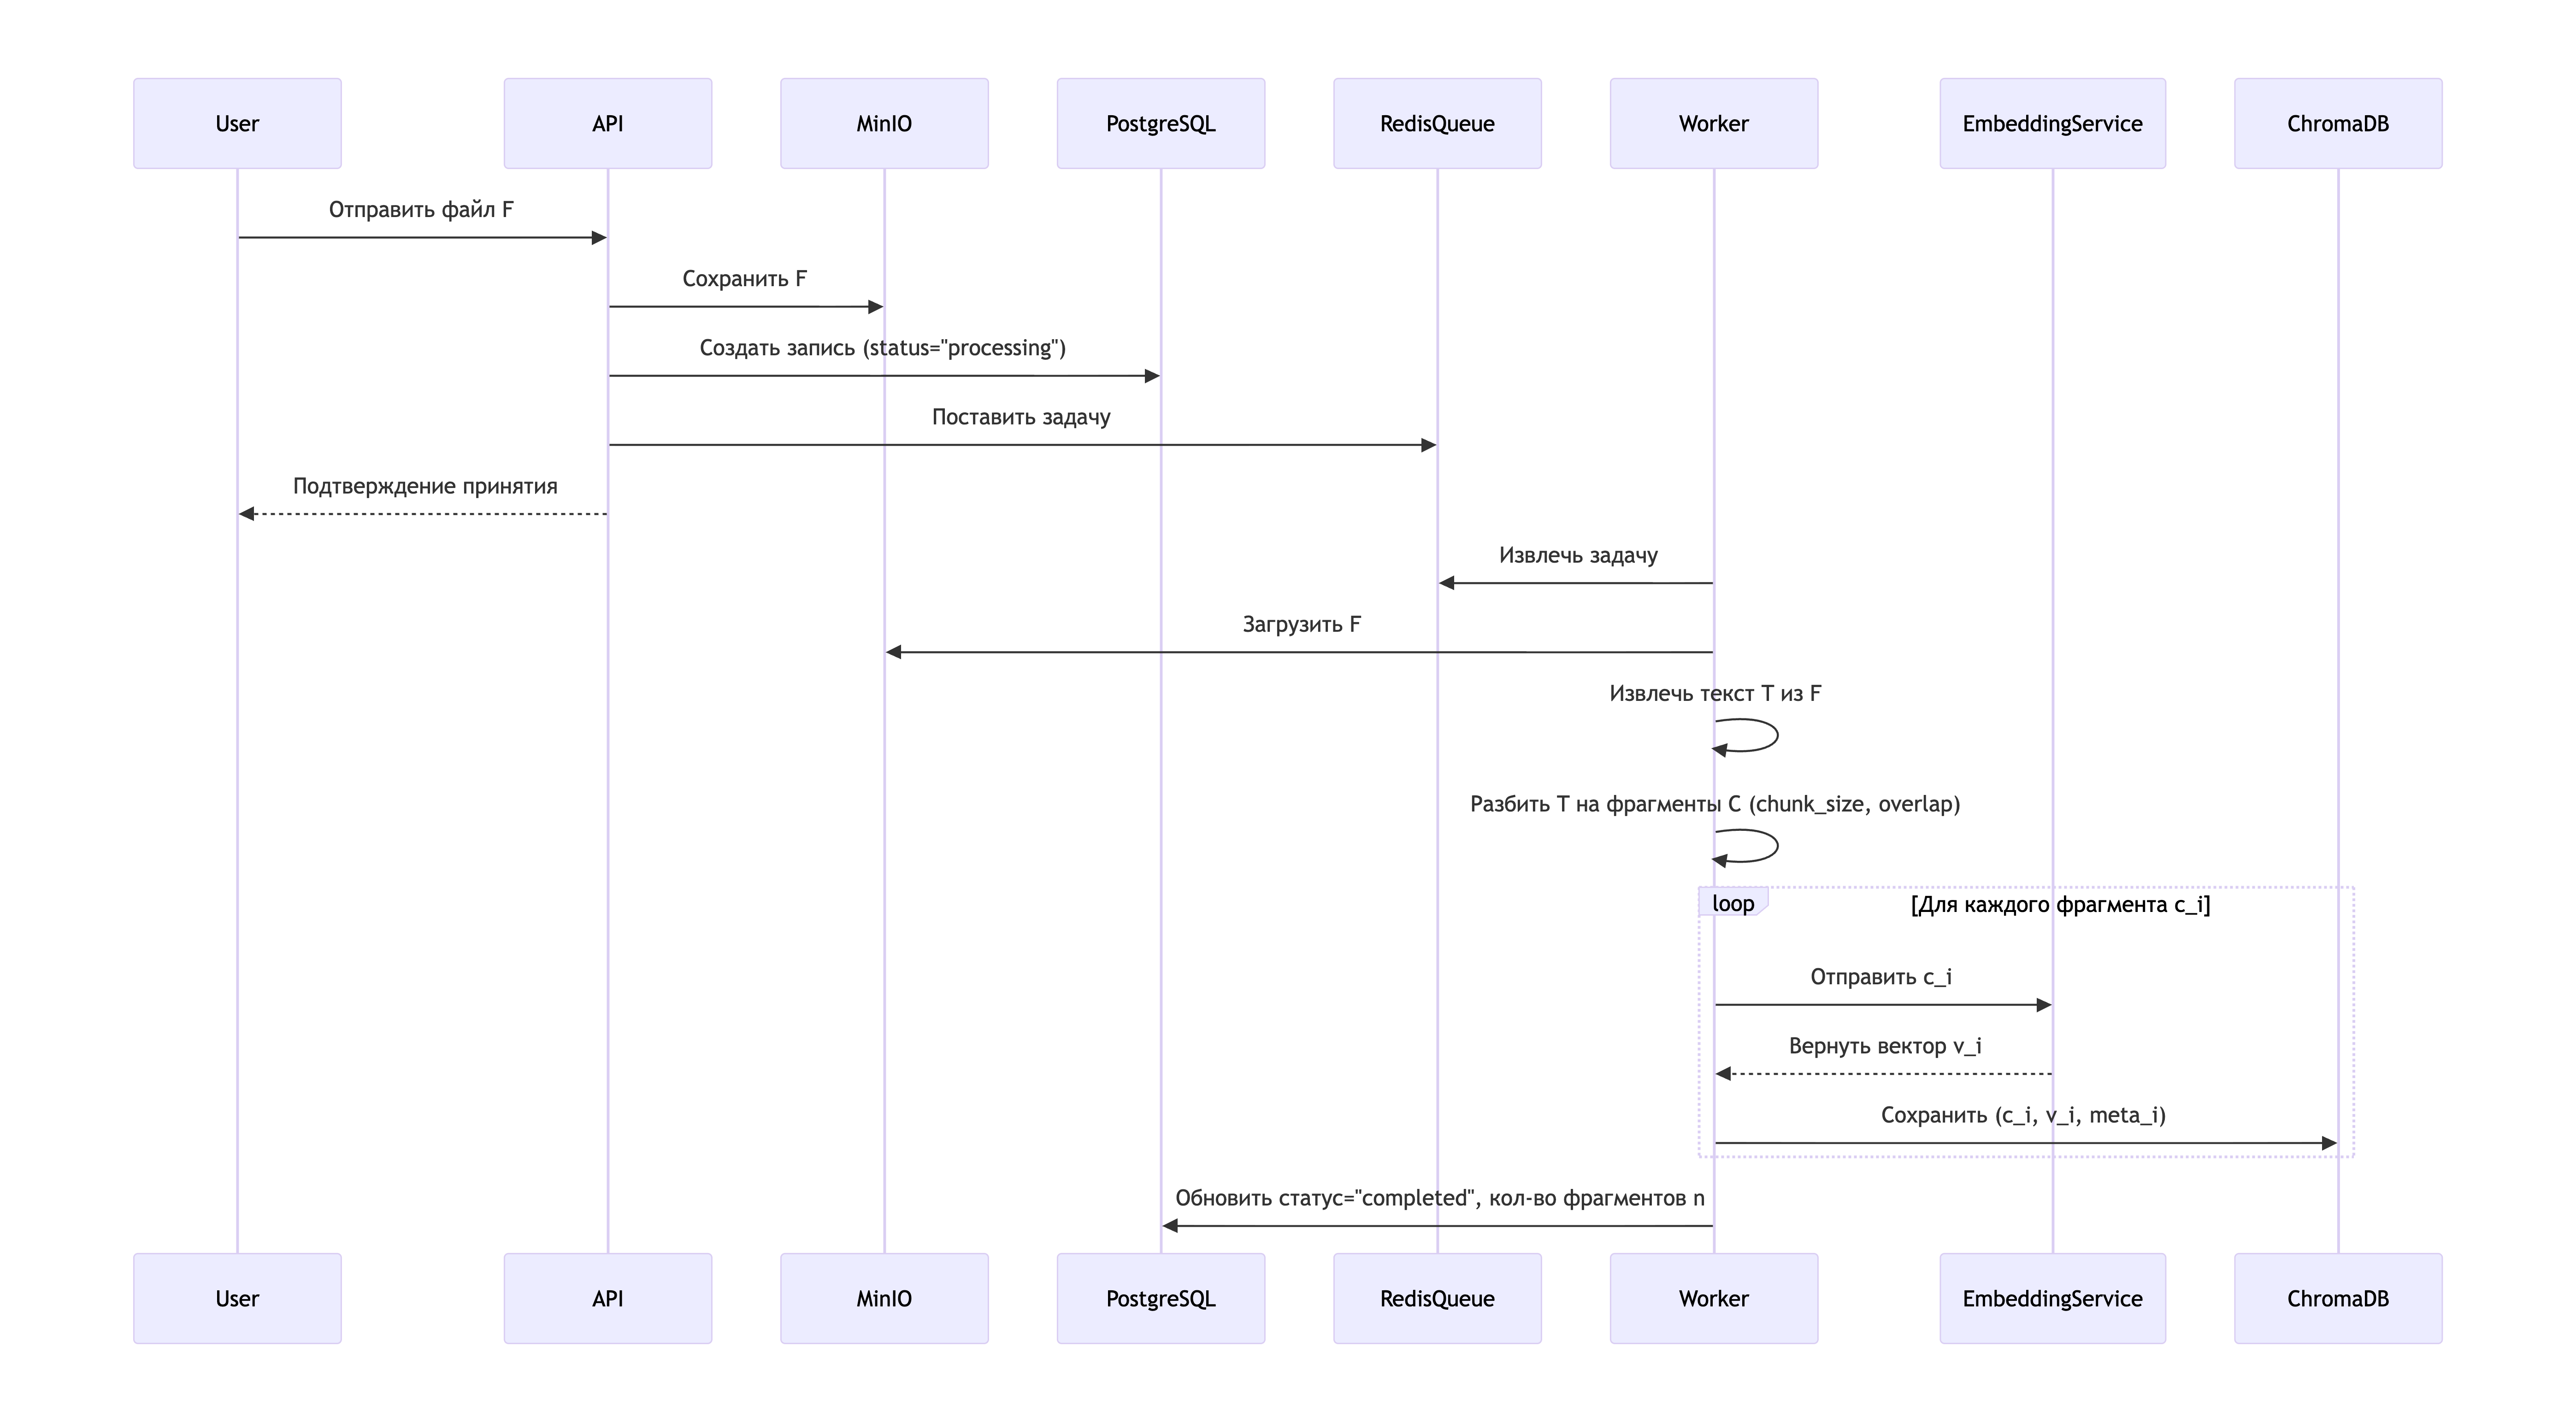
\includegraphics[width=0.9\textwidth]{materials/vectorize.png}
  \caption{Ingest Pipeline flowchart}
  \label{fig:ingestflow}
\end{figure}

Важно отметить, что описанный алгоритм является полностью автоматическим. После того как пользователь загружает документ, ему не нужно предпринимать никаких дополнительных действий: система сама пройдёт все этапы — от сохранения исходного файла в MinIO до финальной индексации векторов в ChromaDB. Статус документа в PostgreSQL последовательно меняется от \texttt{"processing"} к \texttt{"completed"} (или к \texttt{"failed"} в случае ошибки на любом из этапов), что позволяет при необходимости отслеживать прогресс обработки.


\subsection{Алгоритм генерации ответа (RAG Pipeline)}

После того как конвейер поиска (Retrieval Pipeline) вернул упорядоченный список релевантных фрагментов, в дело вступает RAG Service. Его задача — превратить набор разрозненных фрагментов документа в осмысленный, точный и полезный ответ пользователю. Для этого RAG Service формирует специальный промпт, который объединяет контекст (найденные фрагменты) с запросом пользователя, и передаёт этот промпт в языковую модель (LLM).

Промпт $P$ формируется как структурированная конкатенация трёх ключевых частей: системной инструкции, найденных фрагментов контекста и запроса пользователя. Формально это можно записать следующим образом:

\begin{equation}
P = I_{\text{sys}} \;\oplus\; \bigoplus_{i=1}^{K} r_i \;\oplus\; q
\end{equation}

где каждое обозначение имеет конкретный смысл. $I_{\text{sys}}$ — это системная инструкция, которая задаёт модели роль (кем она является) и ограничения (как она должна себя вести). $r_i$ — это $i$-й релевантный фрагмент из множества $R$, то есть тот самый контекст, на который модель должна опираться при ответе. $q$ — исходный запрос пользователя. Символ $\oplus$ обозначает операцию конкатенации (склеивания) текстовых блоков в определённом порядке.

Ниже приведён конкретный шаблон промпта, используемый в системе. Схему следует оставить в том виде, в котором она представлена.

\begin{verbatim}
[Системная инструкция]:
  Ты интеллектуальный ассистент. Отвечай на вопросы строго
  на основе предоставленного контекста. Если ответ не может
  быть получен из контекста — сообщи об этом пользователю.

[Контекст]:
  Фрагмент 1: "..."
  Фрагмент 2: "..."
  ...
  Фрагмент K: "..."

[Вопрос пользователя]:
  {q}

[Ответ]: <генерируется языковой моделью>
\end{verbatim}

Важно обратить внимание на ключевое требование, заложенное в системную инструкцию: отвечать строго на основе предоставленного контекста, а не на основе собственных знаний модели. Это требование — центральный механизм борьбы с галлюцинациями языковых моделей. Если в переданных фрагментах нет информации, необходимой для ответа на вопрос, модель должна честно сообщить об этом пользователю, а не пытаться придумать правдоподобный, но ложный ответ.

После того как языковая модель сгенерировала ответ, он возвращается пользователю через пользовательский интерфейс. Кроме того, система сохраняет пару (запрос пользователя, сгенерированный ответ) в историю диалога. Это сохранение выполняется через DB Connector Service, который записывает данные в PostgreSQL. Хранение истории диалога необходимо для нескольких целей: во-первых, это позволяет пользователю вернуться к предыдущим обсуждениям; во-вторых, история может использоваться для последующего анализа качества работы системы и для дообучения или тонкой настройки промптов.



\subsection{Агентный цикл (ReAct-паттерн)}

Агентный модуль системы реализован на основе паттерна ReAct (Reasoning + Acting) — одного из наиболее эффективных подходов к построению интеллектуальных агентов на базе больших языковых моделей. Идея паттерна заключается в том, что модель не просто выдаёт ответ за один шаг, а чередует фазы рассуждения (Reasoning) и выполнения действий (Acting). На фазе рассуждения модель анализирует, что ей уже известно и чего ещё не хватает. На фазе действия она обращается к внешним инструментам — например, выполняет семантический поиск по документам или обращается к базе данных. Полученные результаты добавляются в контекст, и цикл повторяется. Такой подход позволяет агенту решать многошаговые задачи, требующие последовательного обращения к различным инструментам и постепенного уточнения ответа.

Каждая итерация цикла расширяет контекст языковой модели результатами выполненных действий. Это ключевое свойство: модель не забывает, какой поиск она уже проводила и что из него узнала, а может опираться на эту информацию в следующих шагах рассуждения. Благодаря этому агент способен последовательно уточнять свои рассуждения и в итоге приходить к обоснованному финальному ответу. При обращении к инструменту \texttt{RAGSearch} агент задействует полный конвейер поиска, описанный в разделе 5.

Ниже приведено формальное описание алгоритма агентного цикла. Схему следует оставить в том виде, в котором она представлена.

\begin{verbatim}
Вход:  запрос пользователя q
Выход: финальный ответ A

Алгоритм (итеративный цикл):

Повторять:
  1. Thought:
     LLM анализирует текущее состояние задачи и рассуждает,
     достаточно ли имеющейся информации для ответа.

  2. Если информации достаточно:
     → Action: FinalAnswer
     → Вернуть ответ пользователю. Завершить цикл.

  3. Если требуется дополнительная информация:
     → Action: выбор инструмента из доступного набора:
         - RAGSearch(query)  — семантический поиск по документам
         - иные инструменты (внешние API и пр.)

  4. Observation:
     Выполнить выбранный инструмент, получить результат.
     Добавить результат в контекст рассуждения.

  5. Перейти к шагу 1.
\end{verbatim}

Важно подчеркнуть, что применение ReAct-паттерна даёт системе два важнейших преимущества по сравнению с «глупым» однопроходным подходом. Во-первых, это прозрачность: на каждом шаге видно, почему агент принял то или иное решение и к каким выводам пришёл. Во-вторых, это надёжность: агент может осознать, что первого поиска оказалось недостаточно, и выполнить уточняющий поиск с другими ключевыми словами, или признать, что нужной информации в документах просто нет — и честно сообщить об этом пользователю. Именно на этом паттерне, в частности, основан механизм самокоррекции (Self-Heal) при генерации SQL-запросов: если сгенерированный запрос вызвал ошибку в базе данных, агент получает текст ошибки в Observation и на следующей итерации может исправить запрос.


\subsection{Метрики оценки качества LLM-моделей}

Для количественной оценки качества генерации SQL-запросов использовался набор метрик, отражающих различные аспекты корректности ответа: от строгого совпадения с эталоном до фактической корректности результата выполнения запроса. Такой подход позволяет комплексно оценить поведение моделей, учитывая как синтаксическую, так и семантическую составляющие.

Ключевой метрикой является точность выполнения (Execution Accuracy, EA), которая измеряет долю запросов, успешно выполненных без ошибок и вернувших корректный результат. Формально данная метрика определяется следующим образом:

\begin{equation}
EA = \frac{1}{N} \sum_{i=1}^{N} \mathbb{I}\big( \text{Exec}(q_i) = \text{Exec}(q_i^{*}) \big)
\end{equation}

где $N$ — общее количество тестовых запросов, $q_i$ — сгенерированный SQL-запрос, $q_i^{*}$ — эталонный запрос, а функция $\text{Exec}(\cdot)$ возвращает результат выполнения запроса. Индикаторная функция $\mathbb{I}$ принимает значение 1 в случае совпадения результатов и 0 в противном случае.

Дополнительно используется метрика точного совпадения SQL-текста (Exact Matching Accuracy), которая проверяет полное текстовое совпадение с эталонным запросом:

\begin{equation}
EM = \frac{1}{N} \sum_{i=1}^{N} \mathbb{I}(q_i = q_i^{*})
\end{equation}

Данная метрика является наиболее строгой, поскольку даже незначительные отличия в формате или именовании приводят к снижению оценки, несмотря на возможную логическую корректность запроса.

Для более гибкой оценки синтаксической эквивалентности применяется метрика Exact Set Match (ESM), которая сравнивает структурные компоненты SQL-запроса (например, списки столбцов, условия фильтрации и группировки), игнорируя несущественные различия в порядке или оформлении:

\begin{equation}
ESM = \frac{1}{N} \sum_{i=1}^{N} \mathbb{I}\big( \text{Struct}(q_i) = \text{Struct}(q_i^{*}) \big)
\end{equation}

где $\text{Struct}(\cdot)$ — функция, приводящая SQL-запрос к нормализованному структурному представлению.

Отдельное внимание уделяется расширенной метрике Intelligent Execution Accuracy (IEA), которая представляет собой модификацию Execution Accuracy с учётом допустимых различий в формате результата. В отличие от строгой EA, данная метрика сравнивает результаты с учётом нормализации:

\begin{equation}
IEA = \frac{1}{N} \sum_{i=1}^{N} \mathbb{I}\big( \text{Norm}(\text{Exec}(q_i)) = \text{Norm}(\text{Exec}(q_i^{*})) \big)
\end{equation}

где $\text{Norm}(\cdot)$ — функция нормализации, устраняющая различия в именах колонок, порядке столбцов, форматировании чисел и незначительных числовых погрешностях.

Применение данной метрики позволяет более точно оценить реальную полезность модели, поскольку в практических задачах важна корректность результата, а не строгое совпадение синтаксиса.
